\chapter{MATERIALS AND METHODS}

\section{Experimental Data Preparation}
\subsection{Data Acquisition}
Extracellular metabolomics data is obtained from Cakar's Lab \cite{arslan2018physiological}.Briefly, they perform ethyl methane sulfonate (EMS) mutagenesis  on the prototrophic \emph{Saccharomyces cerevisiae} strain CEN.PK 113-7D (MATa, MAL2-8c, SUC2) to increase the genetic diversity as an evolutionary engineering selection strategy. Cells were inoculated in 2\% Yeast Minimal Media (YMM), and the extracellular concentrations of glucose, ethanol, glycerol and acetate were measured at different time points. OD\textsubscript{600} values were determined by a spectrophotometer. Additionally, cell dry weight analysis was conducted to determine biomass production. Acquired extracellular metabolite concentrations, OD\textsubscript{600} values and dry weights of the reference strain (without mutagenesis) were used in this study are collected in Table \ref{table:experimental_data} and Table \ref{table:experimental_OD600s_and_growths}.

\begin{table}[H]
\caption[Measured OD\textsubscript{600} and cell dry weight values of reference strain \cite{surmeli2019evolutionary}]{Measured OD\textsubscript{600} and cell dry weight values of reference strain \cite{surmeli2019evolutionary}.}
\begin{center}
  \begin{tabular}{|c|c|c|c|}
 \hline
  \textbf{Time (h)} & \textbf{OD600} & \textbf{ln(OD600)} & \textbf{Cell DW (g/L)} \\
  \hline
  0                 & 0.21           & -1.560647748       & -                      \\
  3                 & 0.53           & -0.634878272       & -                      \\
  6                 & 1.76           & 0.565313809        & 0.9                    \\
  7.5               & 2.66           & 0.978326123        & -                      \\
  9                 & 4.46           & 1.495148766        & 1.9                    \\
  12                & 5.31           & 1.669591835        & -                      \\
  15                & 5.88           & 1.771556762        & -                      \\
  18                & 5.83           & 1.763017           & 2.32                   \\
  21                & 6.07           & 1.803358605        & -                      \\
  24                & 5.87           & 1.769854634        & -                      \\
  30                & 6.14           & 1.814824742        & 2.26                   \\
  40                & 6.44           & 1.86252854         & -                      \\
  46                & 6.36           & 1.850028377        & -                      \\
  50                & 6.3            & 1.840549633        & -                      \\
  54                & 6.55           & 1.87946505         & -                      \\
  63                & 6.54           & 1.877937165        & -                      \\
  67                & 6.88           & 1.928618652        & -                      \\
  72                & 6.97           & 1.941615225        & 2.66                  \\
   \hline
  \end{tabular}
\label{table:experimental_OD600s_and_growths}
\end{center}
\end{table}

\begin{table}[H]
\caption[Measurements of extracellular concentrations \cite{surmeli2019evolutionary}]{Measurements of extracellular concentrations \cite{surmeli2019evolutionary}.}
\begin{center}
\begin{tabular}{|c|c|c|c|c|}
   \hline
  \textbf{Time(h)} & \textbf{Glucose(g/L)} & \textbf{Ethanol(g/L)} & \textbf{Glycerol(g/L)} & \textbf{Acetate(g/L)} \\
    \hline
  0                 & 19.99            & 0                & 0                 & 1.08             \\
  3                 & 17.98            & 0.58             & 0.02              & 1.24             \\
  6                 & 15.85            & 1.2              & 0.06              & 1.16             \\
  9                 & 12.21            & 3.39             & 0.18              & 1.37             \\
  12                & 9.18             & 7.97             & 0.61              & 2.45             \\
  15                & 0.4              & 8.17             & 0.69              & 2.46             \\
  27                & 0                & 8.28             & 0.76              & 2.6              \\
  46                & 0                & 8                & 0.77              & 2.45             \\
  50                & 0                & 6.62             & 0.64              & 2.02             \\
  54                & 0                & 5.74             & 0.55              & 1.73             \\
  58                & 0                & 5.46             & 0.54              & 1.74             \\
  72                & 0                & 3.72             & 0.49              & 1.33            \\
   \hline
\end{tabular}
\label{table:experimental_data}
\end{center}
\end{table}


\subsection{Determination of Rates}
As the slope in the curve of lnOD\textsubscript{600} as a function of time gives the growth rates of cells, natural logarithm of OD\textsubscript{600} values were calculated to obtain specific growth rates by using the equation \ref{eq:growthrates}.
  \begin{equation}
      \ \mu = \frac{\Delta \ln{OD_{600}}}{\Delta t}
      \label{eq:growthrates}
  \end{equation}

In order to determine uptake and secretion rates of the metabolites, the steady-state assumption is applied in three hours intervals as the shortest measured time-points. Missing data on cell dry weights are estimated from the OD\textsubscript{600} values, and these cell dry weight data is used to calculate fluxes (in the unit of mmol/gDWh). Measurement of the cell dry weight at the 3rd hour was crucial for the steady-state assumption, however data was not available from the experiments. Curve trend of the OD\textsubscript{600} plot is used as a guide to estimate cell dry weight (Figure \ref{fig:GrowthGraphs}) \hl{Need a method here: Estimation approach, maybe regression or curve fitting?}. Calculated flux values can be found in the Table \ref{table:calculated_fluxes}.
\begin{figure}[H]
  \begin{center}
  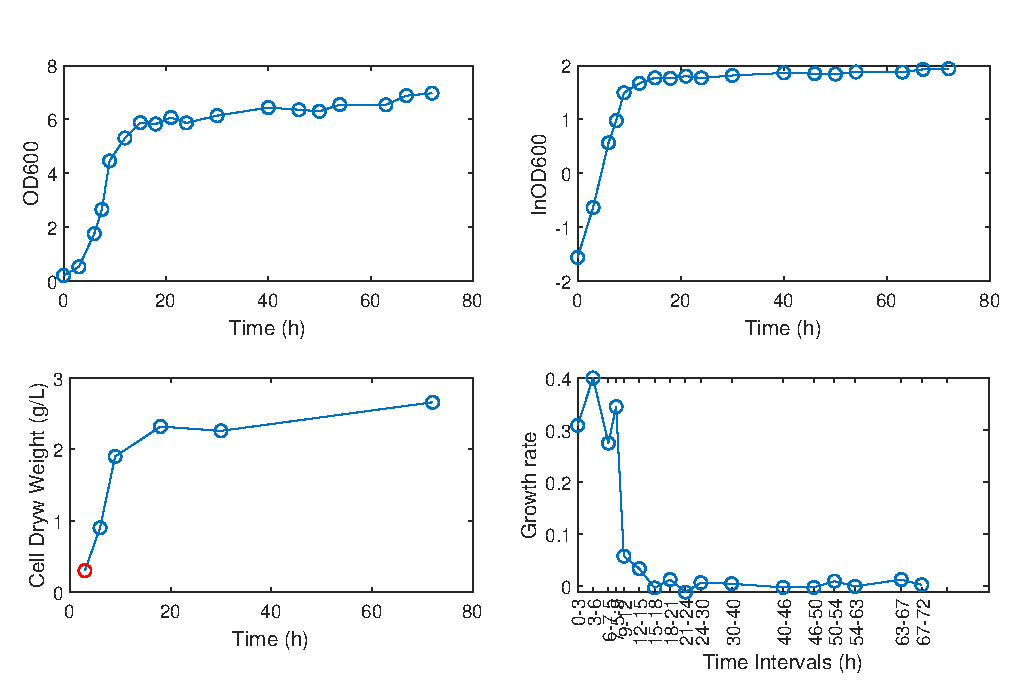
\includegraphics[width=1\columnwidth]{GrowthGraphsSmall.eps}
  \end{center}
  \caption[OD\textsubscript{600}, lnOD\textsubscript{600}, cell dry weights and growth rates]{OD\textsubscript{600}, lnOD\textsubscript{600}, cell dry weights and growth rates graphs. Estimated missing cell dry weight data is shown in red color.}
\label{fig:GrowthGraphs}
\end{figure}

\begin{table}[thbp]
\vskip\baselineskip
\caption[Calculated flux values]{Calculated flux values.}
\begin{center}
  \begin{tabular}{cccccc}
  \multicolumn{1}{l}{\textbf{Time}} & \multicolumn{4}{c}{\textbf{Metabolite fluxes in mmol/gDWh}}                & \textbf{Growth h-1} \\
  \textbf{}                         & \textbf{Glucose} & \textbf{Ethanol} & \textbf{Glycerol} & \textbf{Acetate} & \textbf{Biomass}    \\
  0-3                               & -12.3963884      & 13.98837518      & 0.24131           & 2.960496         & 0.30859             \\
  3-6                               & -4.378823762     & 4.984363569      & 0.160873          & -0.49342         & 0.400064
  \end{tabular}
\label{table:calculated_fluxes}
\end{center}
\end{table}


\section{Model Selection}
iAN50 \cite{nilsson2016metabolic}, a stoichiometric model of intermediary metabolism including glycolysis, the pentose phosphate pathway (PPP), anaerobic excretion, citric acid cycle (TCA cycle), oxidative phosphorylation, and uptake pathways for galactose, ethanol and acetate is used to simulate batch conditions. The model was implemented based on the first GSMM of yeast, iFF708 \cite{forster2003genome} with the addition of the yeast intermediary metabolism from the RAVEN toolbox \cite{agren2013raven}, and finally curated using the KEGG database \cite{kanehisa2000kegg}.

Biomass equation (Eq. \ref{eq:model_biomass}) in the model was left as a function of sub-reactions, for example protein, lipid, DNA synthesis reactions, so that the coefficients of biomass constituents could be optimized for each FBA simulation.
\begin{multline}
  0.5185\ \textrm{Glycogen} + 0.0234\ \textrm{Trehalose} + 0.8079\ \textrm{Mannan} + 1.1348\ \textrm{Glucan} \\
  + 0.1966\ \textrm{DNA} + 0.012\ \textrm{DNA} +  4.14\ \textrm{Protein} + 0.0269\ \textrm{Lipid} + 35.3630 \ \textrm{Maintainance} \\
  = \textrm{BIOMASS}
   \label{eq:model_biomass}
\end{multline}

Enzymatic reactions that are found in the model is collected in Table \ref{table:rxns_smallYeast}. In contrast to other GSMM's, each reaction was irreversible in the iAN50. This was achieved by splitting each reversible reaction into two seperate reactions in both directions.

Another reason to select iAN50 is that the total masses of enzymes catalyzing reactions in the GSMM were already estimated, and fluxes through these reactions were constrained to the biologic level, using an approach similar to intracellular crowding method using kinetic parameters \cite{beg2007intracellular, adadi2012prediction}. To clarify the method briefly, a flux value for each reaction was obtained by applying a standart flux balance analysis, and this value was divided by the maximum \emph{in vitro} activity collected from the enzyme database BRENDA \cite{schomburg2012brenda}, and a saturation factor of 0.5 (half) for simplification. Therefore, the mass of the enzymes required for that particular reaction was estimated and the constrains are applied to the corresponding enzymatic reactions.

\begin{table}[H]
\vskip\baselineskip
  \caption[Reaction list in the iAN50 model]{Reaction list in the iAN50 model.}
  \begin{center}
\resizebox{\textwidth}{!}{
\begin{tabular}{p{11cm}p{17cm}p{8cm}lp{5cm}}
\hline
\textbf{NAME}                                                                             & \textbf{EQUATION}                                                                                                                               & \textbf{GENE ASSOCIATION}                                                                                                                                        & \textbf{EC-NUMBER} & \textbf{SUBSYSTEM}                                                          \\ \hline
Hexokinase                                                                                & GLC{[}c{]} + ATP{[}c{]} =\textgreater ADP{[}c{]} + G6P{[}c{]}                                                                                   & YFR053C; YGL253W; YCL040W                                                                                                                                        & 2.7.1.1 OR 2.7.1.2 & Glycolysis                                                                  \\
Glucose-6-phosphate isomerase                                                             & G6P{[}c{]} \textless{}=\textgreater F6P{[}c{]}                                                                                                  & YBR196C                                                                                                                                                          & 5.3.1.9            & Glycolysis                                                                  \\
Phosphofructokinase                                                                       & ATP{[}c{]} + F6P{[}c{]} =\textgreater ADP{[}c{]} + F16P{[}c{]}                                                                                  & YGR240C; YMR205C                                                                                                                                                 & 2.7.1.11           & Glycolysis                                                                  \\
Fructose-1,6-bisphosphatase                                                               & F16P{[}c{]} =\textgreater F6P{[}c{]} + PI{[}c{]}                                                                                                & YLR377C                                                                                                                                                          & 3.1.3.11           & Glycolysis                                                                  \\
Fructose-bisphosphate aldolase                                                            & F16P{[}c{]} \textless{}=\textgreater GA3P{[}c{]} + DHAP{[}c{]}                                                                                  & YKL060C                                                                                                                                                          & 4.1.2.13           & Glycolysis                                                                  \\
Triosephosphate isomerase                                                                 & DHAP{[}c{]} \textless{}=\textgreater GA3P{[}c{]}                                                                                                & YDR050C                                                                                                                                                          & 5.3.1.1            & Glycolysis                                                                  \\
Triosephosphate dehydrogenase                                                             & GA3P{[}c{]} + NAD{[}c{]} + PI{[}c{]} \textless{}=\textgreater P13G{[}c{]} + NADH{[}c{]}                                                         & YJL052W; YJR009C; YGR192C                                                                                                                                        & 1.2.1.12           & Glycolysis                                                                  \\
Phosphoglycerate kinase                                                                   & P13G{[}c{]} + ADP{[}c{]} \textless{}=\textgreater P3G{[}c{]} + ATP{[}c{]}                                                                       & YCR012W                                                                                                                                                          & 2.7.2.3            & Glycolysis                                                                  \\
Phosphoglycerate mutase                                                                   & P3G{[}c{]} \textless{}=\textgreater P2G{[}c{]}                                                                                                  & YKL152C; YDL021W; YOL056W                                                                                                                                        & 5.4.2.11           & Glycolysis                                                                  \\
Enolase                                                                                   & P2G{[}c{]} \textless{}=\textgreater PEP{[}c{]}                                                                                                  & YGR254W; YHR174W; YOR393W; YPL281C; YMR323W                                                                                                                      & 4.2.1.11           & Glycolysis                                                                  \\
Pyruvate kinase                                                                           & ADP{[}c{]} + PEP{[}c{]} =\textgreater ATP{[}c{]} + PYR{[}c{]}                                                                                   & YOR347C; YAL038W                                                                                                                                                 & 2.7.1.40           & Glycolysis                                                                  \\
Glucose-6-phosphate 1-dehydrogenase                                                       & G6P{[}c{]} + NADP{[}c{]} =\textgreater G15L{[}c{]} + NADPH{[}c{]}                                                                               & YNL241C                                                                                                                                                          & 1.1.1.49           & Pentose Phosphate                                                           \\
6-phosphogluconolactonase                                                                 & G15L{[}c{]} =\textgreater P6G{[}c{]}                                                                                                            & YNR034W; YCR073W-A; YHR163W; YGR248W                                                                                                                             & 3.1.1.31           & Pentose Phosphate                                                           \\
6-phosphogluconate dehydrogenase, decarboxylating                                         & P6G{[}c{]} + NADP{[}c{]} =\textgreater CO2{[}c{]} + RU5P{[}c{]} + NADPH{[}c{]}                                                                  & YGR256W; YHR183W                                                                                                                                                 & 1.1.1.44           & Pentose Phosphate                                                           \\
ribose 5-phosphate isomerase                                                              & RU5P{[}c{]} \textless{}=\textgreater R5P{[}c{]}                                                                                                 & YOR095C                                                                                                                                                          & 5.3.1.6            & Pentose Phosphate                                                           \\
Ribulose-phosphate 3-epimerase                                                            & RU5P{[}c{]} \textless{}=\textgreater X5P{[}c{]}                                                                                                 & YJL121C                                                                                                                                                          & 5.1.3.1            & Pentose Phosphate                                                           \\
Transketolase                                                                             & R5P{[}c{]} + X5P{[}c{]} \textless{}=\textgreater GA3P{[}c{]} + S7P{[}c{]}                                                                       & YBR117C; YPR074C                                                                                                                                                 & 2.2.1.1            & Pentose Phosphate                                                           \\
Transaldolase                                                                             & GA3P{[}c{]} + S7P{[}c{]} \textless{}=\textgreater F6P{[}c{]} + E4P{[}c{]}                                                                       & YLR354C                                                                                                                                                          & 2.2.1.2            & Pentose Phosphate                                                           \\
Transketolase                                                                             & E4P{[}c{]} + X5P{[}c{]} \textless{}=\textgreater F6P{[}c{]} + GA3P{[}c{]}                                                                       & YBR117C; YPR074C                                                                                                                                                 & 2.2.1.1            & Pentose Phosphate                                                           \\
Pyruvate carboxylase 1                                                                    & ATP{[}c{]} + CO2{[}c{]} + PYR{[}c{]} =\textgreater ADP{[}c{]} + OAA{[}c{]} + PI{[}c{]}                                                          & YGL062W; YBR218C                                                                                                                                                 & 6.4.1.1            & TCA                                                                         \\
Citrate synthase, mitochondrial                                                           & ACCOA{[}m{]} + OAA{[}m{]} =\textgreater CI{[}m{]} + COA{[}m{]}                                                                                  & YNR001C; YPR001W                                                                                                                                                 & 2.3.3.1            & TCA                                                                         \\
Aconitate hydratase, mitochondrial                                                        & CI{[}m{]} \textless{}=\textgreater ICI{[}m{]}                                                                                                   & YLR304C                                                                                                                                                          & 4.2.1.3            & TCA                                                                         \\
Isocitrate dehydrogenase                                                                  & ICI{[}m{]} + NAD{[}m{]} =\textgreater AKG{[}m{]} + CO2{[}m{]} + NADH{[}m{]}                                                                     & YNL037C; YOR136W                                                                                                                                                 & 1.1.1.41           & TCA                                                                         \\
Isocitrate dehydrogenase {[}NADP{]}, mitochondrial                                        & ICI{[}m{]} + NADP{[}m{]} =\textgreater AKG{[}m{]} + CO2{[}m{]} + NADPH{[}m{]}                                                                   & YDL066W; YLR174W                                                                                                                                                 & 1.1.1.42           & TCA                                                                         \\
Alpha-ketoglutarate dehydrogenase                                                         & AKG{[}m{]} + NAD{[}m{]} + ADP{[}m{]} + PI{[}m{]} =\textgreater CO2{[}m{]} + NADH{[}m{]} + ATP{[}m{]} + SUC{[}m{]}                               & YDR148C; YIL125W                                                                                                                                                 & 1.2.4.2            & TCA                                                                         \\
Succinate dehydrogenase complex                                                           & FAD{[}m{]} + SUC{[}m{]} =\textgreater FADH2{[}m{]} + FUM{[}m{]}                                                                                 & YKL148C; YLL041C                                                                                                                                                 & 1.3.5.1            & TCA                                                                         \\
Fumarate reductase                                                                        & FADH2{[}m{]} + FUM{[}m{]} =\textgreater FAD{[}m{]} + SUC{[}m{]}                                                                                 & YJR051W; YEL047C                                                                                                                                                 & 1.3.1.6            & TCA                                                                         \\
Fumarate hydratase                                                                        & FUM{[}m{]} \textless{}=\textgreater MAL{[}m{]}                                                                                                  & YPL262W                                                                                                                                                          & 4.2.1.2            & TCA                                                                         \\
Malate dehydrogenase                                                                      & MAL{[}m{]} + NAD{[}m{]} \textless{}=\textgreater NADH{[}m{]} + OAA{[}m{]}                                                                       & YKL085W                                                                                                                                                          & 1.1.1.37           & TCA                                                                         \\
Galactokinase                                                                             & GAL{[}c{]} + ATP{[}c{]} =\textgreater GALP{[}c{]} + ADP{[}c{]}                                                                                  &                                                                                                                                                                  & 2.7.1.6            & Galactose metabolism                                                        \\
UDP-glucose 4-epimerase                                                                   & GALUDP{[}c{]} \textless{}=\textgreater GLUUDP{[}c{]}                                                                                            &                                                                                                                                                                  & 5.1.3.2            & Galactose metabolism                                                        \\
Galactose-1-phosphate uridylyltransferase                                                 & GLUUDP{[}c{]} + GALP{[}c{]} \textless{}=\textgreater G1P{[}c{]} + GALUDP{[}c{]}                                                                 &                                                                                                                                                                  & 2.7.7.12           & Galactose metabolism                                                        \\
Phosphoglucomutase-1                                                                      & G1P{[}c{]} \textless{}=\textgreater G6P{[}c{]}                                                                                                  &                                                                                                                                                                  & 5.4.2.2            & Galactose metabolism                                                        \\
glycerol-3-phosphate dehydrogenase                                                        & DHAP{[}c{]} + NADH{[}c{]} =\textgreater GP{[}c{]} + NAD{[}c{]}                                                                                  & YDL022W; YOL059W                                                                                                                                                 & 1.1.1.8            & Anaerobic excretion                                                         \\
sn-glycerol-3-phosphate phosphohydrolase                                                  & GP{[}c{]} =\textgreater GLY{[}c{]} + PI{[}c{]}                                                                                                  & YER062C; YIL053W                                                                                                                                                 & 3.1.3.21           & Anaerobic excretion                                                         \\
Pyruvate decarboxylase                                                                    & PYR{[}c{]} =\textgreater ACA{[}c{]} + CO2{[}c{]}                                                                                                & YGR087C; YLR134W; YLR044C                                                                                                                                        & 4.1.1.1            & Anaerobic excretion                                                         \\
Alcohol dehydrogenase                                                                     & ACA{[}c{]} + NADH{[}c{]} \textless{}=\textgreater ETH{[}c{]} + NAD{[}c{]}                                                                       & YGL256W; YMR303C; YOL086C                                                                                                                                        & 1.1.1.1            & Anaerobic excretion                                                         \\
Aldehyde dehydrogenase                                                                    & ACA{[}c{]} + NADP{[}c{]} =\textgreater AC{[}c{]} + NADPH{[}c{]}                                                                                 & YPL061W                                                                                                                                                          & 1.2.1.3            & Anaerobic excretion                                                         \\
Aldehyde dehydrogenase {[}NAD(P)+{]} 1                                                    & ACA{[}c{]} + NAD{[}c{]} =\textgreater NADH{[}c{]} + AC{[}c{]}                                                                                   & YMR170C; YMR169C; YOR374W; YOR374W; YER073W                                                                                                                      & 1.2.1.5            & Aromatic amino acid biosynthesis \\
Isocitrate lyase                                                                          & ICI{[}m{]} =\textgreater Glyoxylate{[}m{]} + SUC{[}m{]}                                                                                         & YER065C; YPR006C                                                                                                                                                 & 4.1.3.1            & Anaplerotic reactions                                                       \\
Malate synthase 1, glyoxysomal                                                            & ACCOA{[}m{]} + Glyoxylate{[}m{]} =\textgreater COA{[}m{]} + MAL{[}m{]}                                                                          & YIR031C; YNL117W                                                                                                                                                 & 2.3.3.9            & Anaplerotic reactions                                                       \\
NADH-ubiquinone oxidoreductase, mitochondrial ("Complex 1")                               & NADH{[}m{]} + Ubiquinone-9{[}m{]} =\textgreater Ubiquinol{[}m{]} + NAD{[}m{]}                                                                   & YML120C; YMR145C                                                                                                                                                 & 1.6.5.3 (1.6.5.9)  & Oxidative Phosphorylation                                                   \\
External NADH-ubiquinone oxidoreductase 2, mitochondrial ("Complex 1")                    & NADH{[}c{]} + Ubiquinone-9{[}m{]} =\textgreater Ubiquinol{[}m{]} + NAD{[}c{]}                                                                   & YDL085W                                                                                                                                                          & 1.6.5.3 (1.6.5.9)  & Oxidative Phosphorylation                                                   \\
Succinate dehydrogenase {[}ubiquinone{]} cytochrome b subunit, mitochondrial (Complex II) & FADH2{[}m{]} + Ubiquinone-9{[}m{]} \textless{}=\textgreater FAD{[}m{]} + Ubiquinol{[}m{]}                                                       & YKL141W; YDR178W                                                                                                                                                 & 1.3.5.1            & Oxidative Phosphorylation                                                   \\
Cytochrome b-c1 complex subunit Rieske, mitochondrial (complex III)                       & Ubiquinol{[}m{]} + 2 Ferricytochrome\_c{[}m{]} + 1.5 H{[}m{]} =\textgreater Ubiquinone-9{[}m{]} + 2 Ferrocytochrome\_c{[}m{]} + 1.5 HMit{[}m{]} & YEL024W; YBL045C; YHR001W-A; YPR191W; YFR033C; YDR529C; YJL166W; YGR183C                                                                                         & 1.10.2.2           & Oxidative Phosphorylation                                                   \\
Cytochrome c oxidase subunit 1 (Complex IV)                                               & Ferrocytochrome\_c{[}m{]} + 0.25 O2{[}c{]} + 1.5 H{[}m{]} =\textgreater Ferricytochrome\_c{[}m{]} + 1.5 HMit{[}m{]}                             & YNL052W; YIL111W; YLR395C; Q0045; Q0250; YGL187C; YHR051W; YGL191W; YLR038C; YMR256C; YDL067C                                                                    & 1.9.3.1            & Oxidative Phosphorylation                                                   \\
ATP synthase subunit alpha, mitochondrial (Complex V)                                     & ADP{[}m{]} + PI{[}m{]} + 3 HMit{[}m{]} =\textgreater ATP{[}m{]} + 3 H{[}m{]}                                                                    & YBL099W; Q0080; YPL078C; YDR298C; Q0130; Q0085; YJR121W; YKL016C; YDL004W; YDR322C-A; YPL271W; YDR377W; YPR020W; YBR039W; YLR295C; YML081C-A; YOL077W-A; YML042W & 3.6.3.14           & Oxidative Phosphorylation                                                   \\
ATP hydrolysis                                                                            & ATP{[}c{]} =\textgreater ADP{[}c{]} + PI{[}c{]}                                                                                                 &                                                                                                                                                                  &                    & Other                                                                       \\
Pyruvate dehydrogenase complex                                                            & COA{[}m{]} + NAD{[}m{]} + PYR{[}m{]} =\textgreater ACCOA{[}m{]} + CO2{[}m{]} + NADH{[}m{]}                                                      & YER178W; YFL018C; YBR221C                                                                                                                                        & 1.2.4.1            & Other                                                                       \\
Acetyl-coenzyme A synthetase 1                                                            & AC{[}c{]} + 2 ATP{[}c{]} + COA{[}c{]} =\textgreater ACCOA{[}c{]} + 2 ADP{[}c{]} + 2 PI{[}c{]}                                                   & YAL054C; YLR153C                                                                                                                                                 & 6.2.1.1            & Other                                                                       \\
Phosphoenolpyruvate carboxykinase                                                         & ATP{[}c{]} + OAA{[}c{]} =\textgreater ADP{[}c{]} + CO2{[}c{]} + PEP{[}c{]}                                                                      & YKR097W                                                                                                                                                          & 4.1.1.49           & Other                                                                       \\ \hline
\end{tabular}}
\label{table:rxns_smallYeast}
\end{center}
\end{table}


\section{Flux Balance Analysis}
Uptake reaction of glucose with the secretion reactions of glycerol and acetate were constrained according to the calculated flux values in Table \ref{table:calculated_fluxes}, for both time intervals seperately. Since the main goal was to validate model for experimental conditions, ethanol was not constrained in regard to be used as the control metabolite. Experiments were done in fully aerobic conditions, therefore oxygen uptake reaction was set unlimited.

Coefficients of the biomass constituents are defined as the same as the batch conditions in the reference article \cite{nilsson2016metabolic}, for the reason that detailed knowledge is not available in the acquired experimental data. Coefficients for the final biomass equation can be found in the Table \ref{table:biomass_coefficients}.

\begin{table}[H]
\vskip\baselineskip
\caption[Biomass coefficients]{Biomass coefficients that are used in the simulation.}
\begin{center}
  \begin{tabular}{ll}
  \hline
  \textbf{Constituent} & \textbf{Coefficient} \\ \hline
  Protein              & 3.703704             \\
  RNA                  & 0.37037              \\
  DNA                  & 0.018519             \\
  Lipid                & 0.041667             \\
  Glycogen             & 0.030864             \\
  Trehalose            & 0.029214             \\
  Mannan               & 0                    \\
  Glucan               & 2.469136             \\
  Maintainance         & 40                   \\ \hline
  \end{tabular}
\label{table:biomass_coefficients}
\end{center}
\end{table}
For the linear optimization, an implementation of pFBA from the reference publication was performed \cite{nilsson2016metabolic, AvlantGithub}. After solving the system using a linear solver with the objective maximizing growth, the solution was used as a constraint. From that point, a second optimization was run to minimize the sum of all other fluxes.

\section{Visualization of the Model}
The GSMM was visualized in Cytoscape \cite{cline2007integration} using the Fluxviz plug-in \cite{konig2010fluxviz} and the solution fluxes were mapped onto edges. Network was imported in SBML \cite{hucka2018systems} and the flux distributions were imported in csv format.
